%%%%%%%%%%%%%%%%%%%%%%%%%%%%%%%%%%%%%%%%%
% a0poster Landscape Poster
% LaTeX Template
% Version 1.0 (22/06/13)
%
% The a0poster class was created by:
% Gerlinde Kettl and Matthias Weiser (tex@kettl.de)
%
% This template has been downloaded from:
% http://www.LaTeXTemplates.com
%
% License:
% CC BY-NC-SA 3.0 (http://creativecommons.org/licenses/by-nc-sa/3.0/)
%
%%%%%%%%%%%%%%%%%%%%%%%%%%%%%%%%%%%%%%%%%

%-------------------------------------------------------------------------------
%	PACKAGES AND OTHER DOCUMENT CONFIGURATIONS
%-------------------------------------------------------------------------------

\documentclass[a0, landscape]{a0poster}

\usepackage{multicol} % This is so we can have multiple columns of text side-by-side
\columnsep=100pt % This is the amount of white space between the columns in the poster
\columnseprule=3pt % This is the thickness of the black line between the columns in the poster

\usepackage[svgnames]{xcolor} % Specify colors by their 'svgnames', for a full list of all colors available see here: http://www.latextemplates.com/svgnames-colors

%\usepackage{times} % Use the times font
% \usepackage{palatino} % Uncomment to use the Palatino font
% \usepackage{}
\usepackage{fontspec}
\setmainfont{Latin Modern Sans}

\usepackage{graphicx} % Required for including images
\graphicspath{{figures/}} % Location of the graphics files
\usepackage{booktabs} % Top and bottom rules for table
\usepackage[font=small,labelfont=bf]{caption} % Required for specifying captions to tables and figures
\usepackage{amsfonts, amsmath, amsthm, amssymb} % For math fonts, symbols and environments
\usepackage{wrapfig} % Allows wrapping text around tables and figures

\usepackage{listings}
\usepackage{color}

\definecolor{dkgreen}{rgb}{0,0.6,0}
\definecolor{gray}{rgb}{0.5,0.5,0.5}
\definecolor{mauve}{rgb}{0.58,0,0.82}

\lstset{
  %frame=tb,
  language=Python,
  aboveskip=2mm,
  belowskip=0mm,
  showstringspaces=false,
  columns=flexible,
  basicstyle={\small\ttfamily},
  numbers=none,
  numberstyle=\tiny\color{gray},
  keywordstyle=\color{blue},
  commentstyle=\color{dkgreen},
  stringstyle=\color{mauve},
  breaklines=true,
  breakatwhitespace=true,
  tabsize=3,
  framexleftmargin=15pt
  }


\begin{document}

%----------------------------------------------------------------------------------------
%	POSTER HEADER
%----------------------------------------------------------------------------------------

% The header is divided into three boxes:
% The first is 55% wide and houses the title, subtitle, names and university/organization
% The second is 25% wide and houses contact information
% The third is 19% wide and houses a logo for your university/organization or a photo of you
% The widths of these boxes can be easily edited to accommodate your content as you see fit

\begin{minipage}[b]{0.80\linewidth}
\veryHuge \color{NavyBlue} \textbf{PanNeuro: leveraging a community-based approach for big data neuroscience} \color{Black}\\ % Title
%\Huge\textit{An Exploration of Complexity}\\[1cm] % Subtitle
\huge \textbf{Ariel Rokem\textsuperscript{1,2,*}, Joe Hamman \textsuperscript{3}, Ryan Abernathy \textsuperscript{4} \&  Adrienne Fairhall\textsuperscript{2,5}}\\ % Author(s)
\Large 1. The eScience Institute, 2. Computational Neuroscience Center 5. Dept. of Physiology and Biophsyics, Univ. of Washington \\
3. National Center for Atmospheric Research, 4. Earth and Environmental Sciences, Columbia University \\% University/organization
\Large *Contact: \texttt{arokem@uw.edu} $|$ Download: \texttt{http://arokem.org/presentations/brainpi-panneuro-2019}
\end{minipage}
\begin{minipage}[b]{0.19\linewidth}

\includegraphics[width=10cm]{UWlogo.png}

\includegraphics[width=10cm]{small_e_logo_cropped.png}
\end{minipage}

\vspace{0.5cm} % A bit of extra whitespace between the header and poster content

%----------------------------------------------------------------------------------------

\begin{multicols}{3} % This is how many columns your poster will be broken into, a poster with many figures may benefit from less columns whereas a text-heavy poster benefits from more

%----------------------------------------------------------------------------%	Introduction
%----------------------------------------------------------------------------

\section*{Introduction}

\subsection*{Computational and circuit mechanisms underlying rapid learning}
\subsubsection*{NINDS/NIH U19 funded through the BRAIN Initiative}

\begin{minipage}[b]{1\linewidth}
\hfill
\begin{minipage}[]{0.3\linewidth}
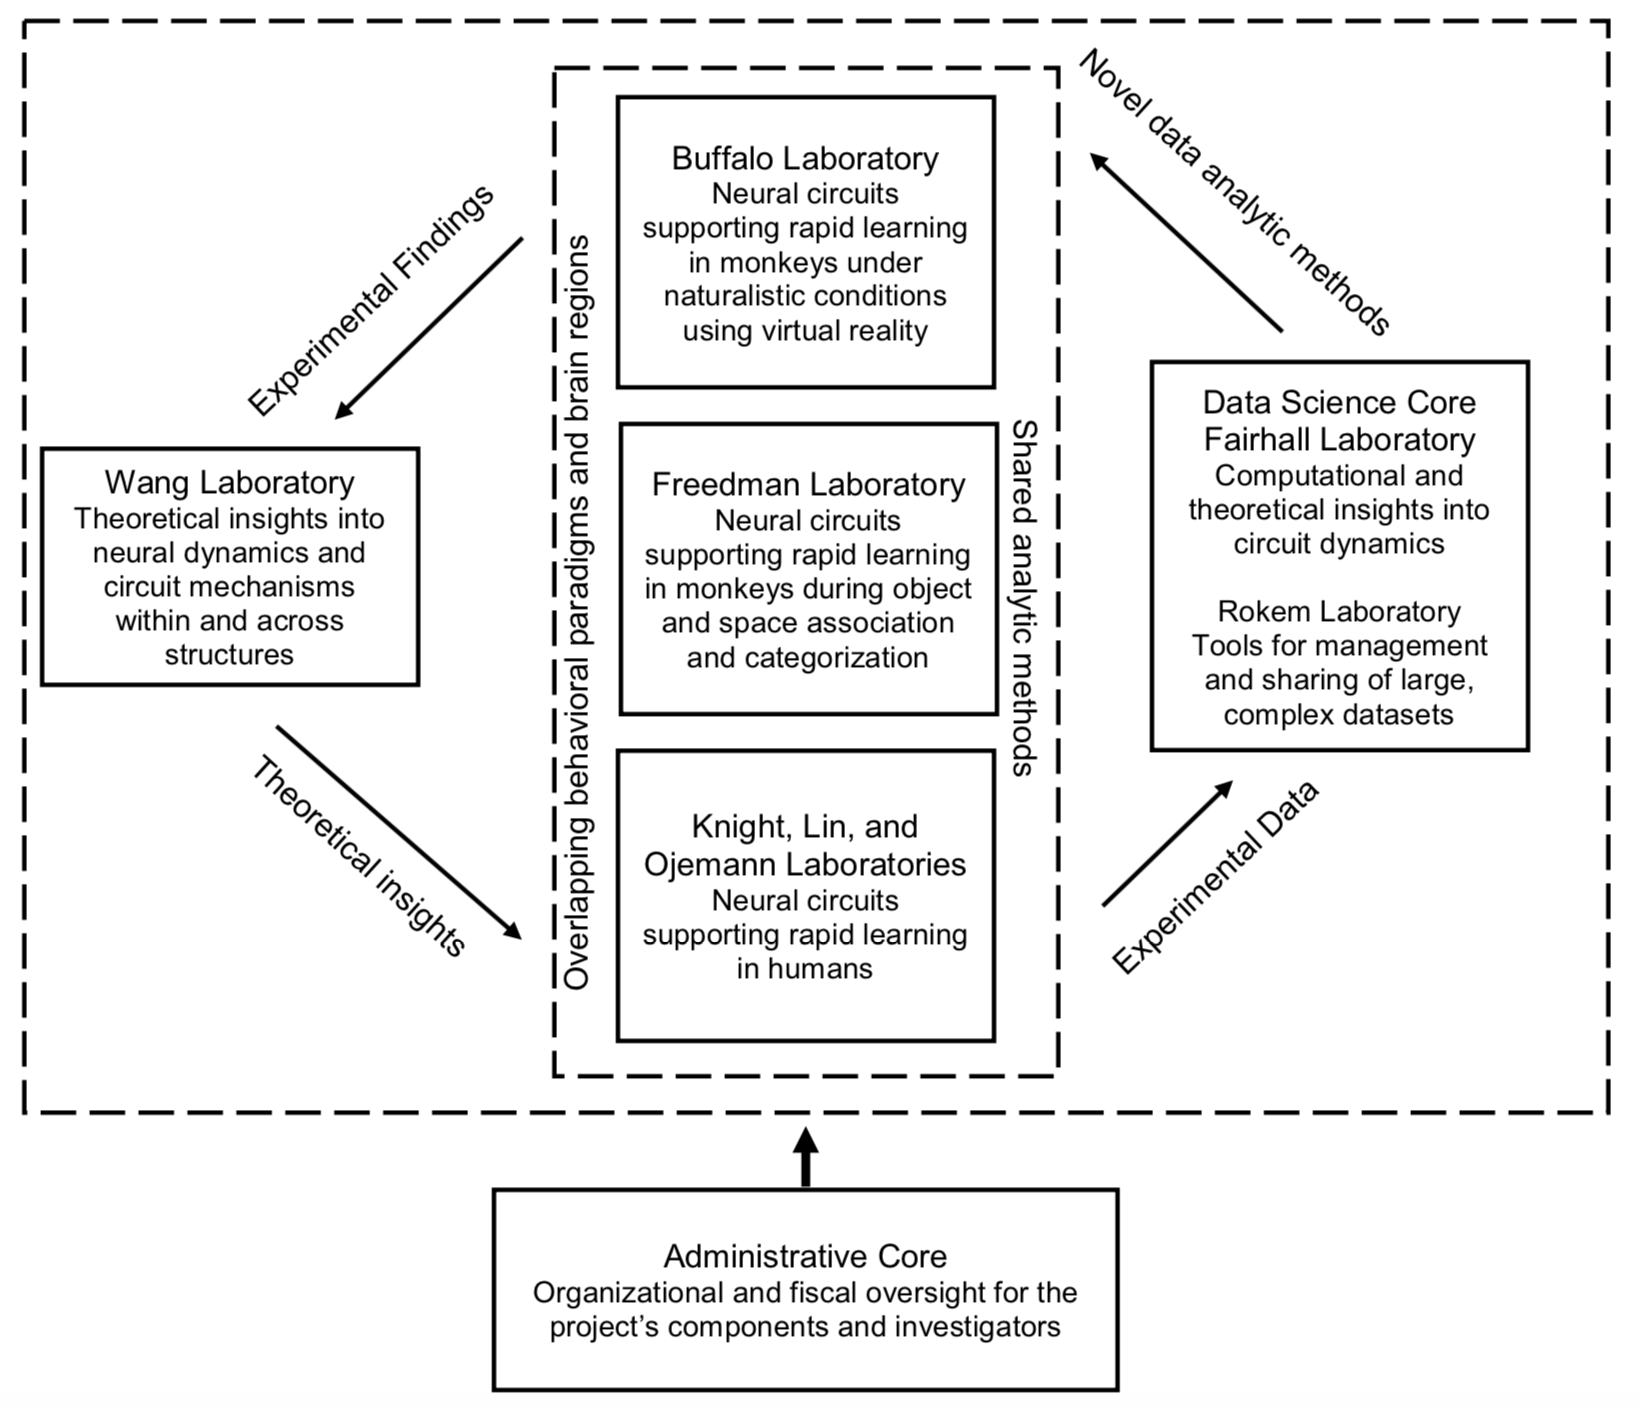
\includegraphics[height=9cm]{u19-collaboration.png}
\end{minipage}
\hfill
\begin{minipage}[]{0.3\linewidth}
\begin{flushleft}
``Learning to learn''\cite{ Harlow1949-bd}
\end{flushleft}
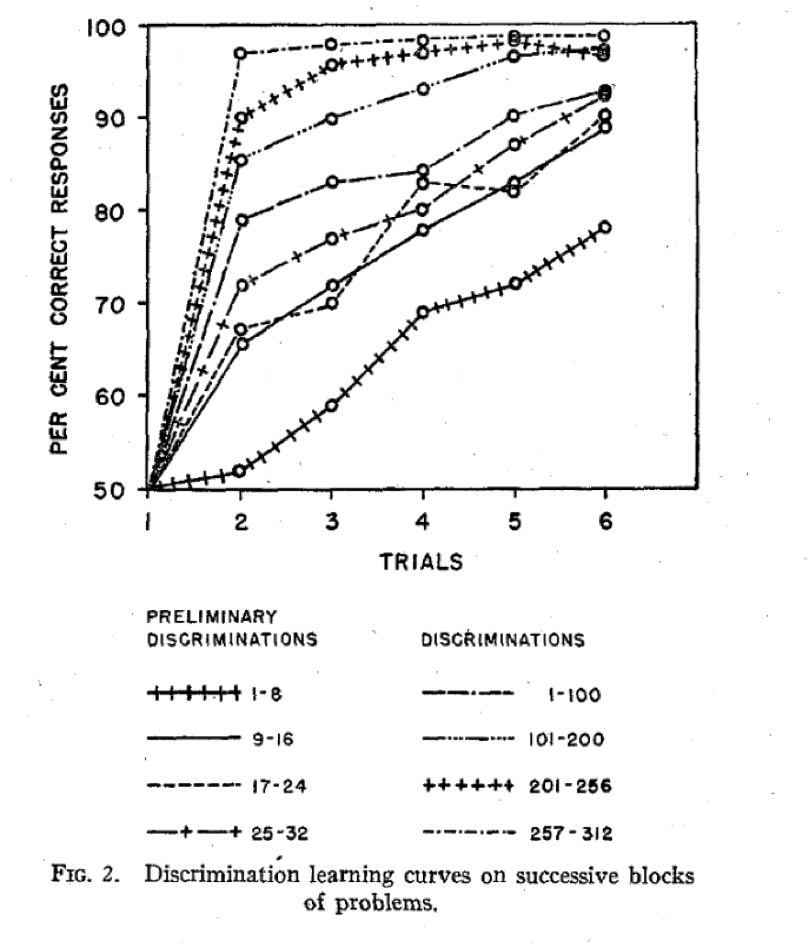
\includegraphics[height=10cm]{harlow49.png}
\end{minipage}
\hfill
\begin{minipage}[]{0.3\linewidth}
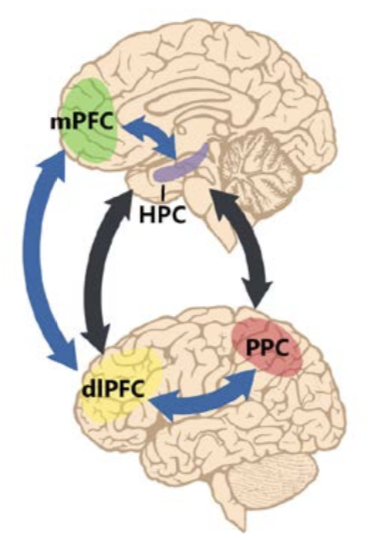
\includegraphics[height=10cm]{circuit-diagram.png}
\end{minipage}
\hfill
\end{minipage}

\subsubsection*{Aims}
\begin{itemize}
\item Identify the neural mechanisms that support schema development and rapid learning in association and categorization paradigms in monkeys and humans.

\item Develop and validate novel techniques for large-scale single unit recordings from multiple distributed regions of the nonhuman and human primate brain, during learning, through reversible inactivation, and during sleep.

\item Generate and test a multi-region computational understanding of circuit mechanisms that underlie schema development and rapid learning.

\end{itemize}


\subsubsection*{High-throughput/resolution recordings in human and non-human primate}

\begin{minipage}[b]{1\linewidth}
\hfill
\begin{minipage}[]{0.3\linewidth}
\begin{flushleft}Multi-channel recordings in monkey\end{flushleft}
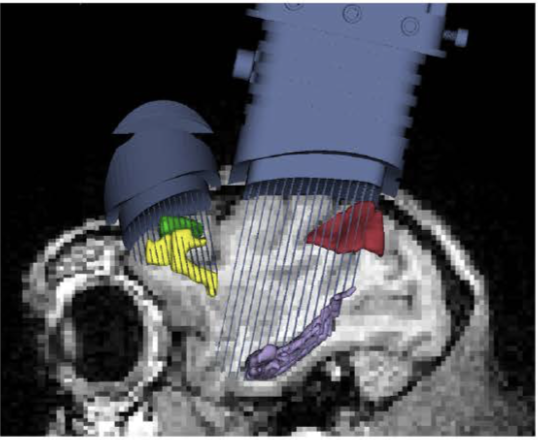
\includegraphics[height=7cm]{nhp-electrodes}
\end{minipage}
\hfill
\begin{minipage}[]{0.2\linewidth}
\begin{flushleft}ECoG recordings in human\end{flushleft}
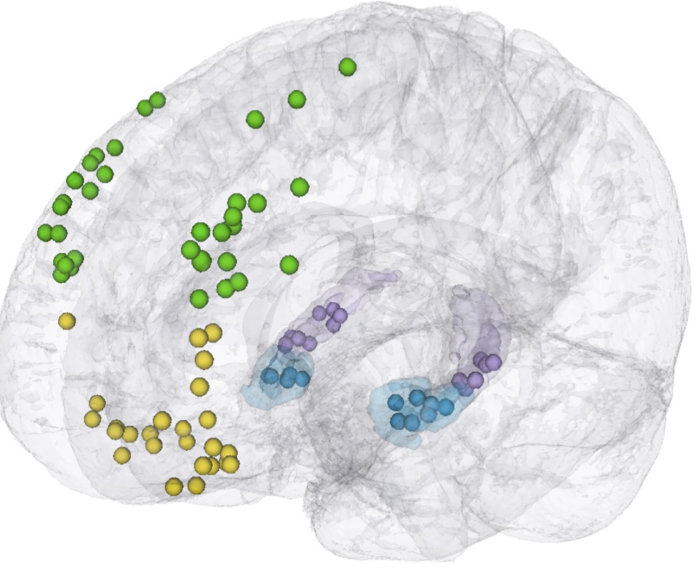
\includegraphics[height=7cm]{ecog-electrodes}
\end{minipage}
\hfill
\begin{minipage}[]{0.3\linewidth}
\begin{flushleft}Single/multi-channel recordings in human\end{flushleft}
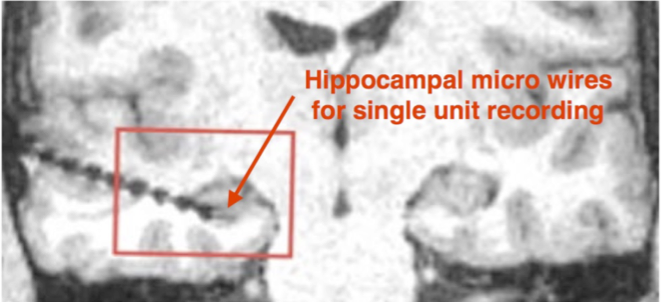
\includegraphics[height=5cm]{depth-electrodes}
\end{minipage}
\hfill
\end{minipage}

\subsubsection*{Same tasks used across species}

\begin{minipage}[b]{1\linewidth}
\begin{minipage}[]{0.4\linewidth}
\begin{flushleft}Variation on WCST\end{flushleft}
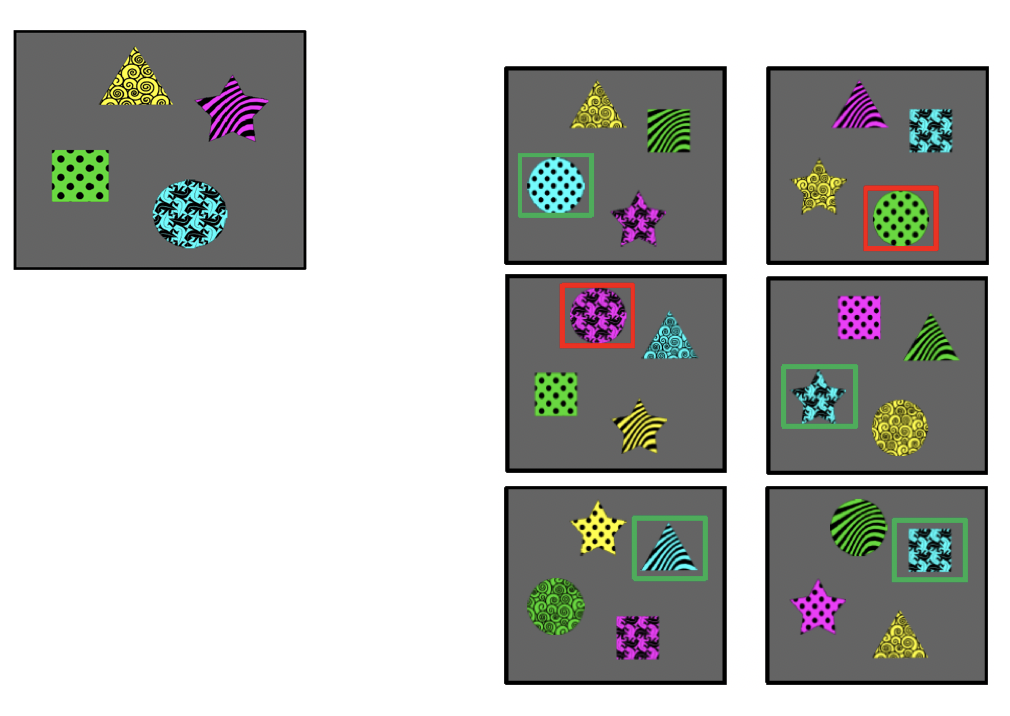
\includegraphics[height=10cm]{wcst}
\end{minipage}
\hfill
\begin{minipage}[]{0.4\linewidth}
\begin{flushleft}Variation on context-dependent learning task \cite{behrens2018cognitive} \end{flushleft}
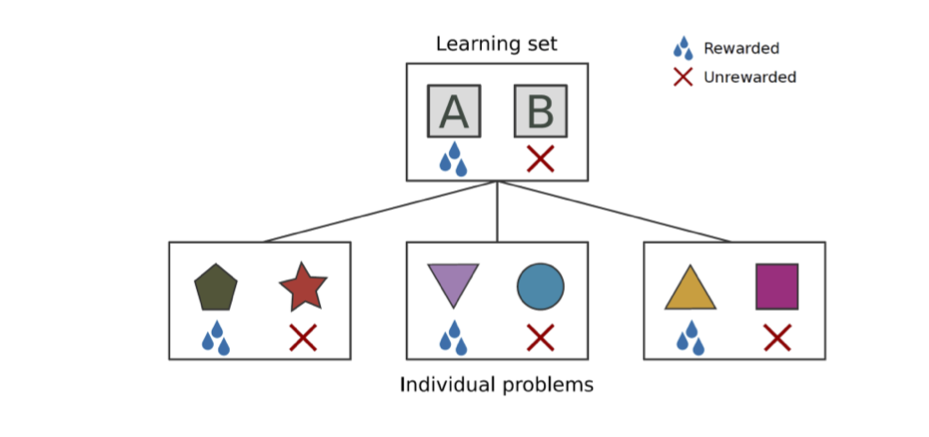
\includegraphics[height=7cm]{behrens-paradigm}
\end{minipage}
\end{minipage}
% \\
% 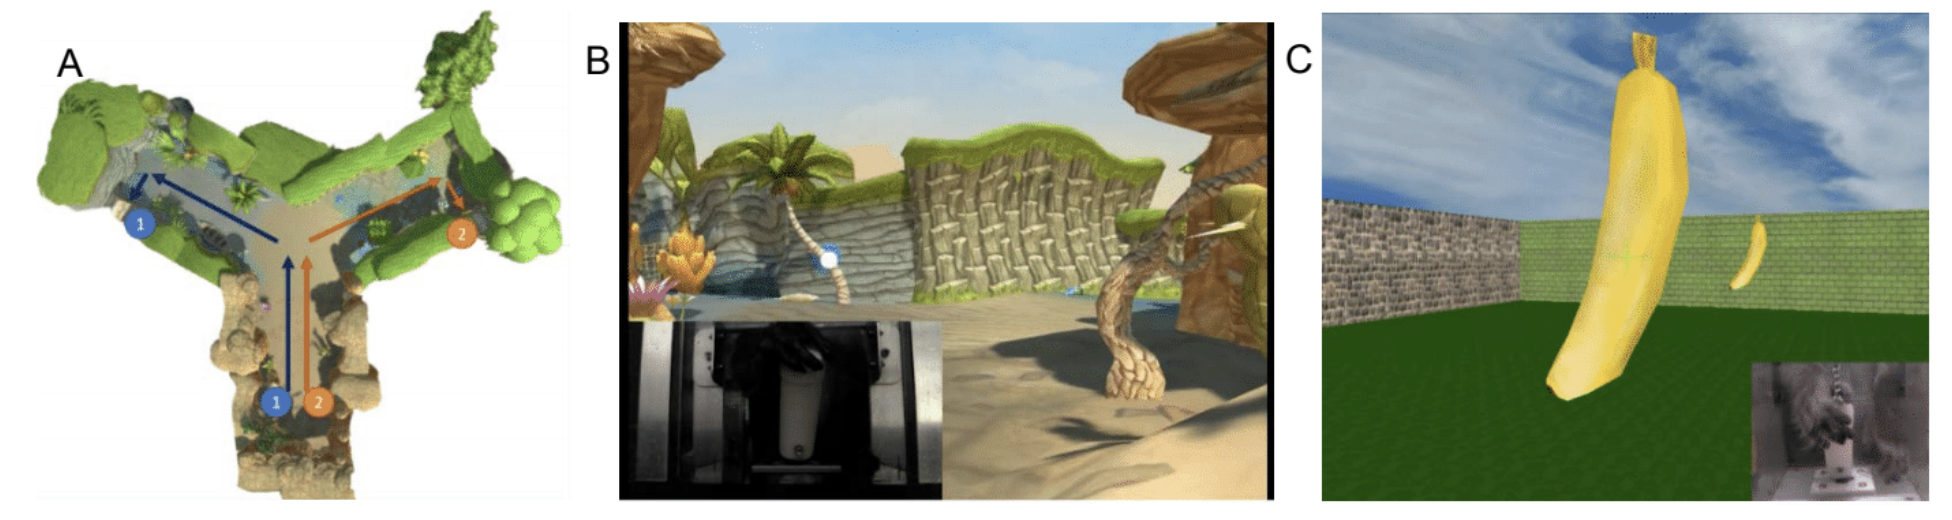
\includegraphics[height=6cm]{vr}

\begin{minipage}[b]{0.45\linewidth}
\subsubsection*{Data types}
\begin{itemize}
\item Behavioral results
\item Non-human primate multichannel recordings
\item Human grid and electrode recordings
\item Model and simulation results
\end{itemize}
\end{minipage}
\hfill
\begin{minipage}[b]{0.45\linewidth}
\subsubsection*{Data volumes}
\begin{itemize}
\item $\sim$5-20 TB/week at steady-state
\item $\sim$1-2 PB to store at steady-state
\item $\sim$10\%-20\% of that needs to be routinely accessed
\end{itemize}
\end{minipage}

\vfill
\columnbreak

%----------------------------------------------------------------------------%
%----------------------------------------------------------------------------
\color{Navy}

\section*{The \emph{PanNeuro} framework}

\subsection*{Inspiration in geoscience big data}
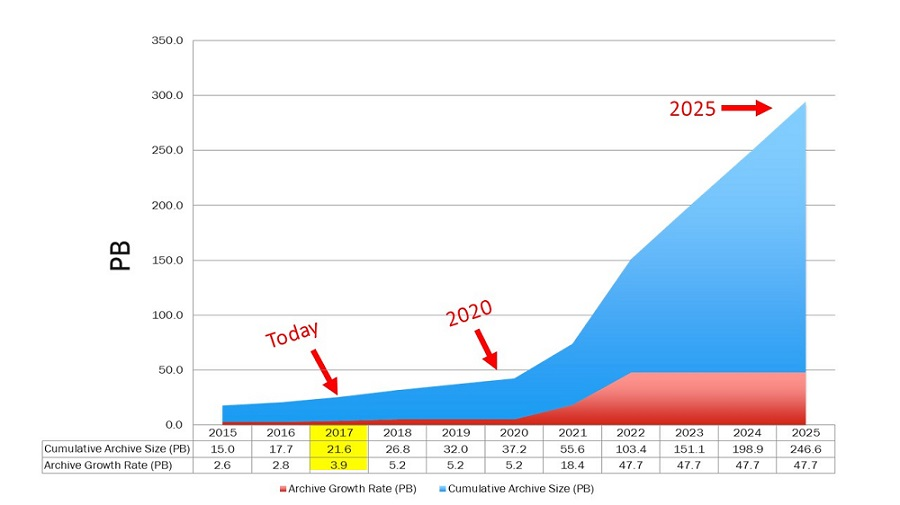
\includegraphics[height=10cm]{EOSDIS_archive_growth_updated_resize}
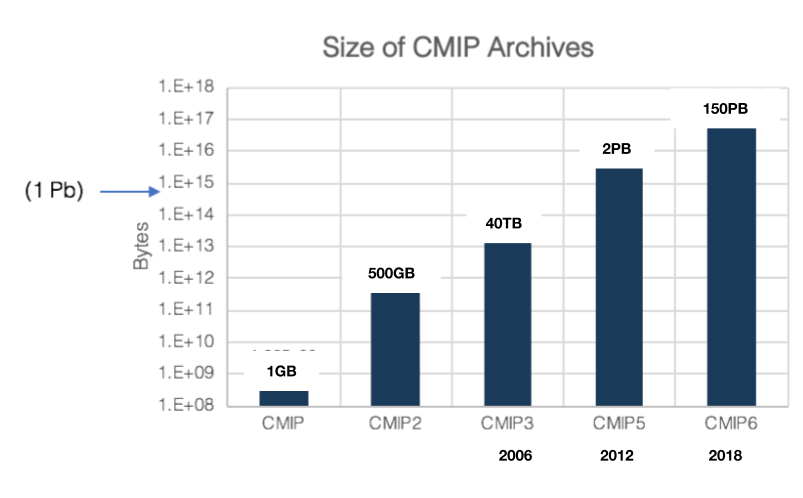
\includegraphics[height=10cm]{cmip-size}

\begin{center}

\includegraphics[height=4cm]{pangeo-logo}\\
\large A community platform for Big Data Geoscience
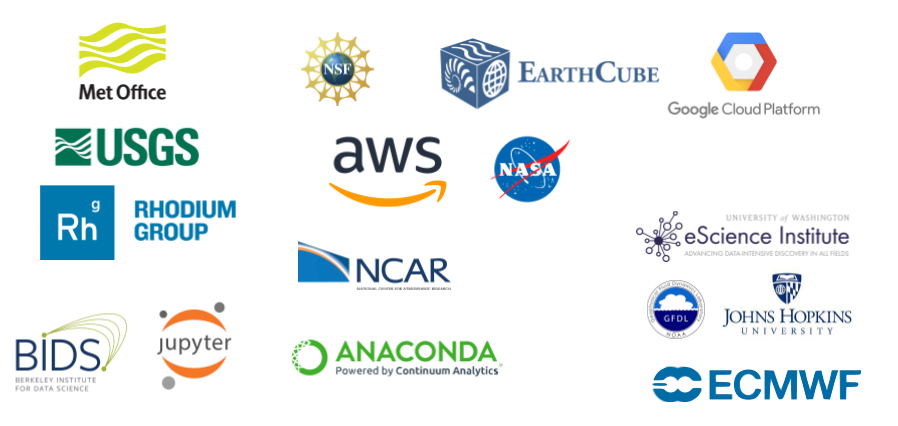
\includegraphics[height=12cm]{pangeo-backers}
\end{center}


\begin{minipage}[b]{0.5\linewidth}
\begin{itemize}
\subsection*{Cloud computing}
\item Bring the compute to the data.
\item Scalable computing.
\item Minimize data duplication.
\item Reproducibility.
\end{itemize}
\end{minipage}
\begin{minipage}[b]{0.5\linewidth}
\subsubsection*{The Pangeo/PanNeuro architecture}
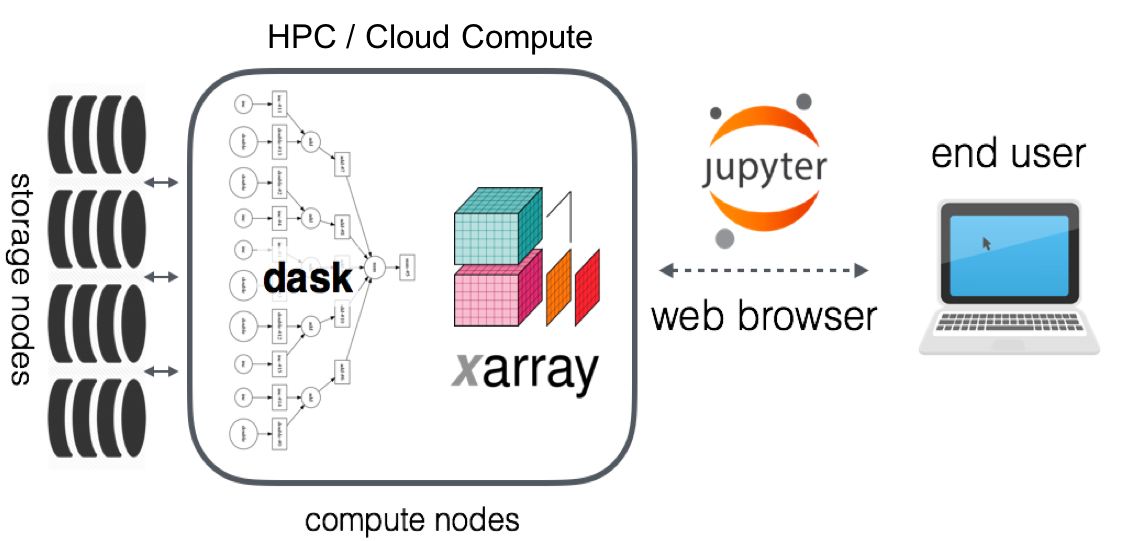
\includegraphics[height=8cm]{pangeo_architecture.png}
\end{minipage}


\subsection*{Scientific computing in Python}
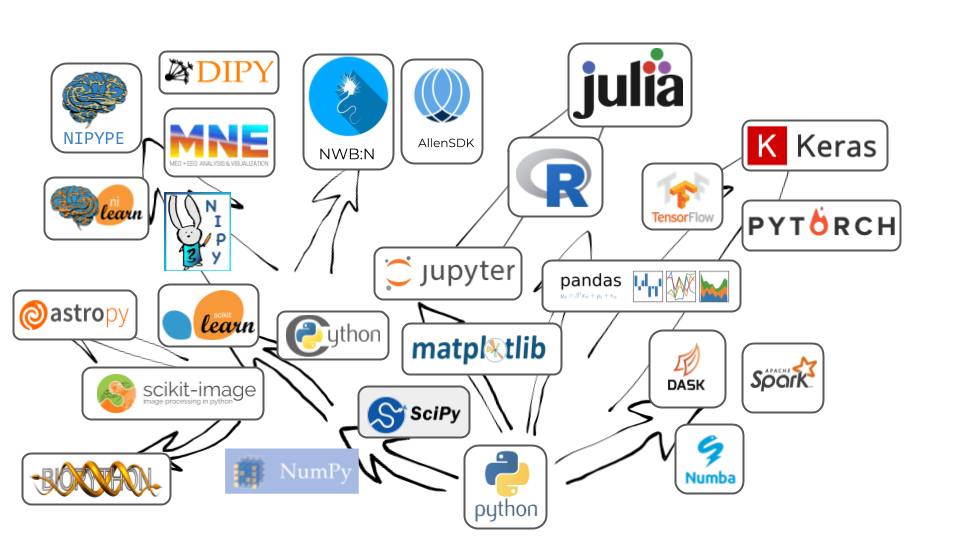
\includegraphics[height=16cm]{python-network25.png}

\vfill
\columnbreak

\subsection*{Jupyter notebook interface}

\begin{itemize}
\item Shareable, reproducible computational narratives
\item Access controlled
\item Scalable cluster accessed through the notebook
\end{itemize}
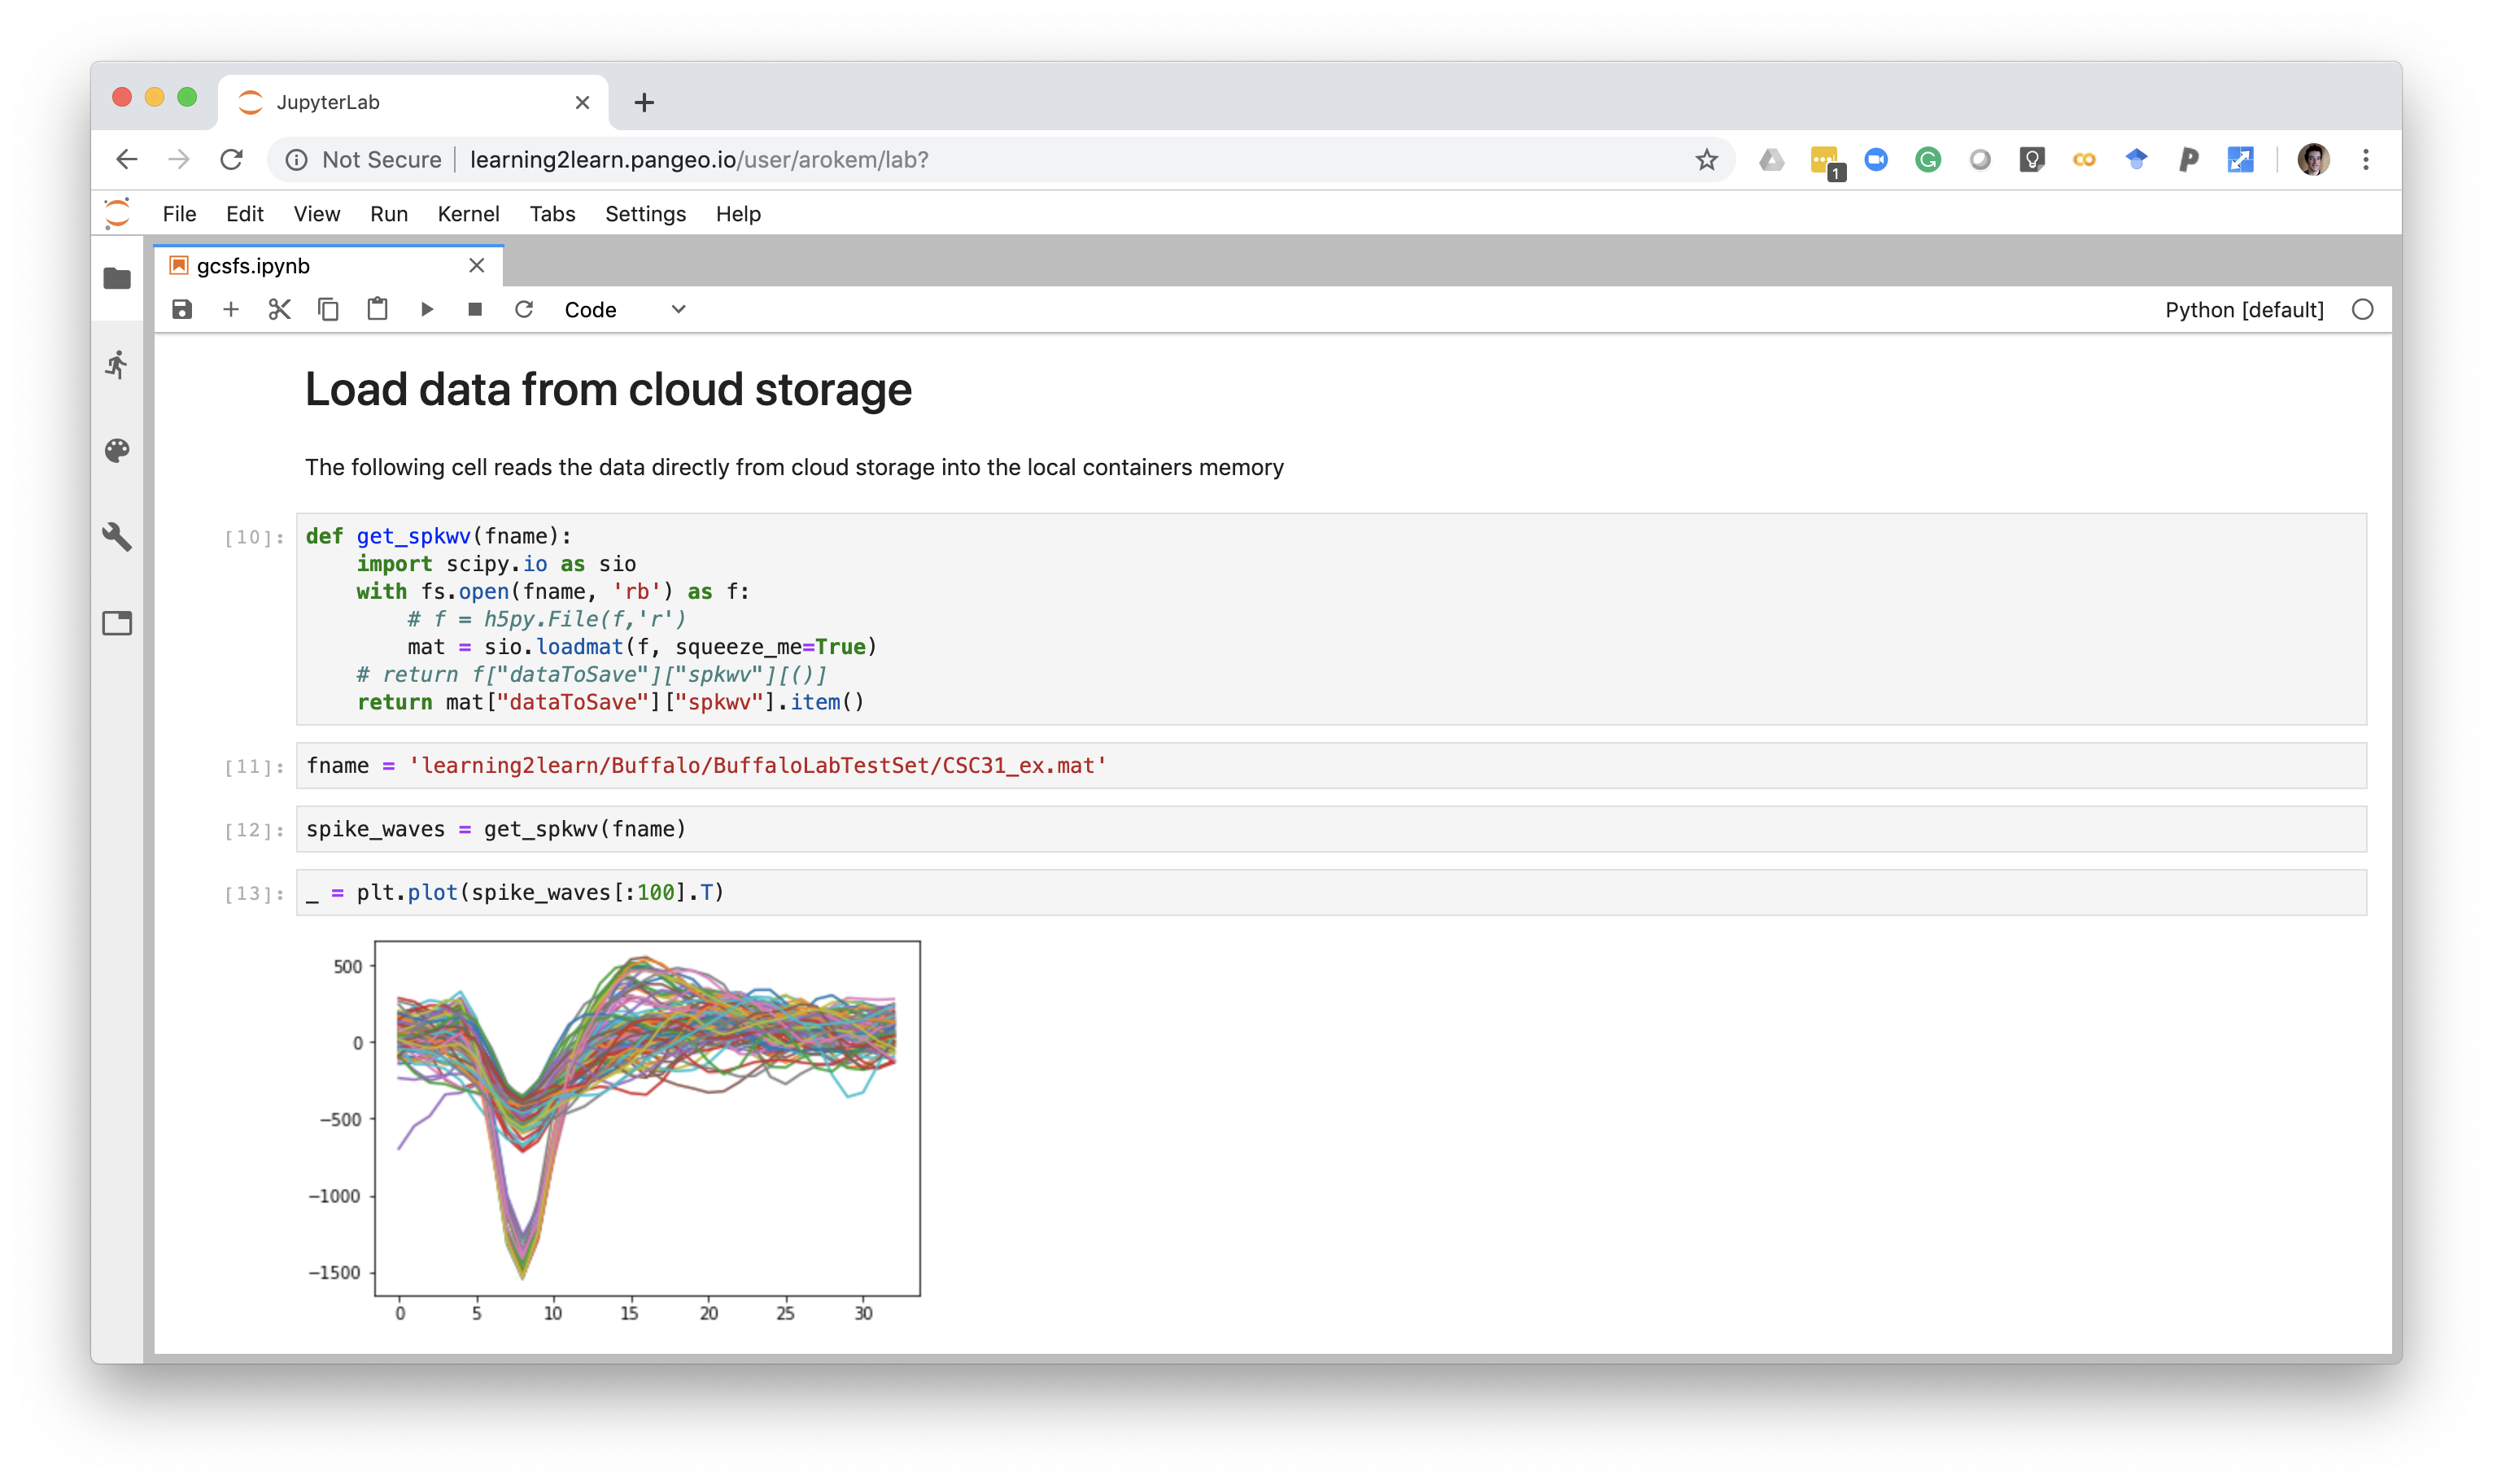
\includegraphics[height=20cm]{notebook_example}


\section*{Try it yourself!}
{\bf \large \texttt{https://learning-2-learn.github.io/panneuro\_binder\_demo}}

%----------------------------------------------------------------------------
%	MATERIALS AND METHODS
%----------------------------------------------------------------------------

\color{SaddleBrown} % SaddleBrown color for the conclusions to make them stand out
\section*{Barriers to adoption}
\begin{itemize}
    \item Concerns about cost
    \item Reluctance to share data
    \item New skills required
    \item The tools are rapidly evolving
    \item Data formats and data standardization
\end{itemize}

\color{DarkSlateGray} % Set the color back to DarkSlateGray for the rest of the content

%---------------------------------------------------------------------------	REFERENCES
%----------------------------------------------------------------------------

\nocite{*} % Print all references regardless of whether they were cited in the poster or not
\bibliographystyle{plain} % Plain referencing style
\footnotesize \bibliography{poster} % Use the example bibliography file sample.bib

%----------------------------------------------------------------------------%	ACKNOWLEDGEMENTS
%----------------------------------------------------------------------------
\subsection*{Acknowledgements} \footnotesize


\includegraphics[height=5cm]{brain-logo.png}

\includegraphics[height=5cm]{NINDS.jpg}\\

\includegraphics[height=3.2cm]{SloanLogo.png}

\includegraphics[height=3.2cm]{MooreFdn.png}

\includegraphics[height=3.2cm]{eSciencelogo.png}
%----------------------------------------------------------------------------

\end{multicols}
\end{document}
